
\subsection{Finite-sample width and coverage on real pools (C2)}
\label{sec:real}
We now fit the adjusters of Sec.~\ref{sec:method} from the labelled draw only and compare each interval with PPI++ \emph{calibrated the same way} (Wald with Wald, $t$ with $t$, bootstrap with bootstrap), paired
on the same draws. The grid covers the four pools of the main text (\texttt{census\_income}, \texttt{gene\_expression}, \texttt{galaxies}, \texttt{forest}), $n\in\{50,100,200,500,1000\}$ and 2000 repetitions per cell,
with $N=\min(\text{pool},10^4)$; the three further pools are in the appendix. Over all 270 cells (pool, $n$, adjuster, calibration), 252 are significantly
\emph{wider} than the like-for-like PPI++ (the confidence interval of the paired width ratio lies above 1), 9 are indistinguishable from parity and 9 are significantly narrower.
All nine narrower cells are at $n=1000$ on \texttt{forest} (gradient boosting 0.995, isotonic 0.997) and \texttt{gene\_expression} (cubic polynomial 0.998); the largest saving is 0.55\%. The cells are not independent: the three calibrations use the same draws, so the nine are three (pool, adjuster) combinations.
So \emph{on these real pools and for the mean, no adjuster shortens the interval in any practically relevant way}.

\begin{figure}[t]
\centering
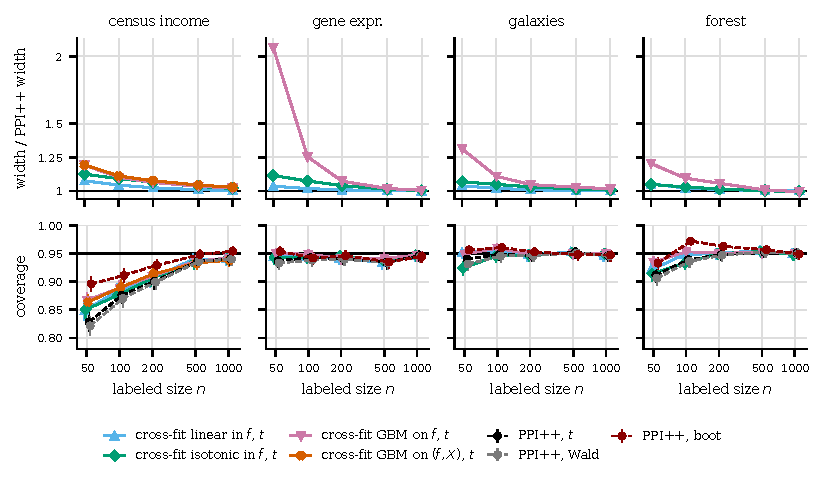
\includegraphics[width=\linewidth]{figures/fig_c2_real.pdf}
\caption{Mean estimation on four real pools. Top: paired width ratio of each cross-fitted adjuster to PPI++ calibrated the same way ($t$ quantile; $<1$ is narrower), geometric mean with 95\% band, log axis; the cubic and the Wald and bootstrap variants are in the delivered summaries. Bottom: coverage of the 95\% interval with Wilson bars; PPI++ (Wald, $t$, bootstrap) dashed.
$n=50$ to $1000$, 2000 repetitions per cell, i.i.d.\ with replacement from the pool, $N=\min(\text{pool},10^4)$, truth the pool mean.}
\label{fig:c2}
\end{figure}

The loss is the estimation cost anticipated in Sec.~\ref{sec:theory} and falls with $n$. At $n=50$ the like-for-like ratios of the affine-in-$f$ adjuster, which is PPI++ up to cross-fitting, are 1.04 to 1.08;
for isotonic recalibration 1.05 to 1.13, for gradient boosting on $f$ 1.20 to 2.06 (\texttt{gene\_expression}). They shrink with $n$ but stay at or above 1.00 for all but the nine cells above (at most 1.03 at $n=1000$).
On \texttt{census\_income}, the pool with features, adjusters that use $X$ do not help: at $n=200$, linear in $(f,X)$ is 1.027 and boosting on $(f,X)$ 1.076, against a population headroom of 0.5\% (Sec.~\ref{sec:headroom}),
which is smaller than the estimation cost, and not recovered within $n\le1000$ (1.005 and 1.027 there). Using studentised bootstrap in place of Wald for both sides gives the same pattern (82 of 90 bootstrap cells significantly wider, 3 narrower).
The same holds as the labelled-to-unlabelled ratio varies: on \texttt{census\_income} at $n=200$ with $N=200$, $2000$ and $20000$, boosting on $(f,X)$ is 1.029, 1.068 and 1.078 times as wide as PPI++, linear in $(f,X)$ 1.010, 1.024 and 1.027;
a larger unlabelled set makes the affine tuning harder to beat, in line with the factor $1/(1+\rho)$ in~\eqref{eq:var}.

\emph{Coverage.} Coverage does not rescue the adjusters: where PPI++ undercovers, the adjusters undercover too, usually slightly less. On \texttt{census\_income} at $n=200$ Wald coverage is 0.899 for PPI++ and 0.902 to 0.912 for the adjusters;
at $n=1000$ 0.940 for PPI++ and 0.938 to 0.943 for the adjusters. Calibrating by the bootstrap lifts PPI++ itself to 0.929 at $n=200$ and 0.954 at $n=1000$, and that calibration is not free: the bootstrap interval for PPI++ is 37\% wider than its Wald interval at $n=50$ and 15\% wider at $n=200$ on \texttt{census\_income}.
The like-for-like comparison is the honest one, since the Wald baseline is narrow partly because it undercovers.
Classical (labelled-only) intervals are 1.1 to 1.5 times wider than PPI++ on \texttt{forest}, \texttt{galaxies} and \texttt{census\_income} at all sizes, and 2.5 to 3.4 times on \texttt{gene\_expression},
so the large gain in this setting is from PPI++'s use of the predictor, not from anything added on top of it.
